\chapter{Phân tích và thiết kế hệ thống}

\section{Xây dựng Multilayer Neural Network}
\subsection{Feature Selection - Dữ liệu luyện tập}
Một trong những yếu tố hết sức quan trọng trong Machine Learning đó chính Feature. 
Feature chính là các giá trị thuộc tính đại diện cho tập dữ liệu luyện tập, ví dụ 
chúng ta có tập dữ liệu về loài chim thì có thể feature chính là các thông số 
về độ dài sải cánh, màu lông, vùng sinh sống... Một giải thuật có thể học được 
"kinh nghiệm" nhanh hay chậm, chính xác hay sai lệch phụ thuộc rất nhiều vào yếu 
tố feature. Vì vậy quá trình khai phá dữ liệu là hết sức cần chú ý.\\\\
Tập dữ liệu về các phiên giao dịch BITCOIN được thu thập từ ngày 20/2/2015 đến 
ngày 29/10/2016 và có tổng cộng 29634 phiên giao dịch.\\\\
Gọi S là đại diện cho một phiên giao dịch, các feature được xây dựng như sau:
\begin{itemize}
    \item 10 feature RDP: $\{ \: loop\{ RDP_1(S_{i+j})\}_i \: \}_j$ Với 
    $i \in [0:9], \: j \in [0:29634]$
    \item 1 feature SO. Với $ j \in [0:29625] $:\\
    \[
        \{ \%K_j = \frac{P(j+9)-L_{10}}{H_{10}-L_{10}} \}_j
    \]
    \item 1 feature ROC. Với $ j \in [9:29634] $:\\ 
    \[
        \{ ROC_{10}(j)= \frac{P(j) - P(j-9)}{P(j-9)} \}_j
    \]
\end{itemize}
Ở đây, ta đã chủ ý chọn mỗi feature vector được hình thành bởi 10 phiên giao 
dịch. Các giá trị SO và ROC đều được tính trong thời gian là 10 phiên giao dịch.
Sau khi đã có feature, ta cần label để phân lớp tập luện tập. Ở đây đơn giản, 
nếu giá BITCOIN ở phiên thứ 11 lớn hơn phiên thứ 10 thì label sẽ là 1, ngược
lại sẽ là 0. (Phiên 11 chính là phiên thứ 1 của nhóm 10 phiên liền sau nhóm 
10 phiên hiện đang xét).\\\\
\[
    label_i = \bigg \{ _{0 \quad if \: P_i(10) \: \leq \: P_{i+1}(1)} ^{1 \quad if \: P_i(10) \: > \: P_{i+1}(1)}
\]
\subsection{Training - Học giải thuật}
Bên cạnh chạy giải thuật Multilayer Neural Network, chúng ta sẽ chạy các giải 
thuật khác nhằm so sánh và đánh giá giải thuật chính.\\\\
Các giải thuật được chọn chạy:\\
\begin{itemize}
\item Multilayer Neural Network - MNN
\item Support Vector Machine - SVM
\item K-Nearest Neighbors - KNN
\item Logistic Regression - LR
\end{itemize}
Sau khi chạy xong ta ghi nhận kết quả của các giải thuật được đề cập dưới dạng 
các tham số đánh giá sau:\\
\begin{itemize}
\item Accuracy
\item Recall
\item Precision
\end{itemize}
\subsection{Validation - Đánh giá giải thuật}
Để có được kết quả đánh giá, chúng ta sẽ chia tập dữ liệu ra hai phần:
\begin{itemize}
\item Training data: chiếm 7/10 tổng số dữ liệu, dùng để chạy trong quá trình 
học của giải thuật.
\item Validation data: chiếm 3/10 tổng số dữ liệu, dùng để chạy trong quá trình 
đánh giá giải thuật.
\end{itemize}
Kết quả chạy giải thuật:\\
\begin{table}[h]
\centering
\begin{tabular}{ |c|c|c|c|c| }
\hline
 & KNN & LR & SVM & MNN \\
\hline
Accuracy & 62.93\% & 66.24\% & 66.40\% & 69.86\% &
\hline
Precision & 44.69\% & 18.18\% & 0\% & 60.50\% &
\hline
Recall & 43.62\% & 0.15\% & 0\% & 29.55\% &
\hline
\end{tabular}
\caption{Bảng đánh giá}
\end{table}\\
Trước tiên theo bảng đánh giá, ta có các giải thuật LR và SVM cho kết quả Accuracy
là gần khoảng 66\%, nhưng khi nhìn và chi tiết các giá trị Precision và Recall 
ta nhận thấy các giải thuật này hầu như chỉ dự đoán kết quả là Down cho tất cả 
trường hợp. Điều này hoàn toàn không có ý nghĩa để dự đoán đầu tư.\\\\
Xét đến KNN và MNN, đối với KNN ta có thể thấy giải thuật có xu hướng cân bằng 
các giá trị Accuracy, Precision và Recall. Nhưng đối với MNN, giải thuật có xu 
hướng tối ưu hóa Accuracy và Precision. Vậy câu hỏi đặt ra ở đây là kết quả nào 
có giá trị đầu tư hơn?\\\\
Chú ý đến Recall, dựa theo định nghĩa thì Recall có thể hiểu nếu trong thực tế 
có 10 phiên là Up thì KNN sẽ dự đoán đúng khoảng 4 lần và MNN sẽ dự đoán đúng 
khoảng 3 lần. Nhìn thoáng qua có vẻ như Recall cao thì sẽ có ý nghĩa trong việc 
đầu tư hơn, nhưng hay khoan kết luận.\\\\
Xét đến Precision, ta có thể hiểu Precision là, với 10 lần dự đoán sẽ có phiên 
Up thì KNN sẽ đúng khoảng 4 lần và MNN sẽ dự đoán đúng 6 lần. Giả sử, mức độ tin 
tưởng của chúng ta vào hệ thống là 100\%, cứ mỗi lần hệ thống dự đoán có phiên Up 
thì ta sẽ bỏ tiền đầu tư. Điều đó đồng nghĩa, nếu theo KNN sẽ có 6 lần ta chịu 
lỗ vì hệ thống dự đoán sai và với MNN thì ta sẽ có 4 lần ta chịu lỗ.\\\\
Quay lại với Recall, giá trị này không đo đạt được việc chúng ta sẽ lợi nhuận 
hoặc thua lỗ ra sao mà thực ra là giá trị đo đạt khả năng tận dụng cơ hội của hệ 
thống.\\\\
Tới lúc này, ta có thể kết luận, bộ giá trị chiếm ưu tiên cao hơn sẽ là Accuracy 
và Precision. Điều đó cũng có nghĩa là giải thuật Multilayer Neural Network nên 
là lựa chọn để tiếp cận giải quyết vấn đề này.\\\\

\section{Xây dựng hệ thống - Web Application}
\subsection{Tổng quan hệ thống}
Hệ thống được xem xét và được thiết kế với 3 khối server chức năng:
\begin{itemize}
\item Hệ thống Machine Learning server
\item Hệ thống Backend server
\item Hệ thống UI Frontend server
\end{itemize}
Các khối hệ thống giao tiếp với nhau bằng API và Socket - đối với các chức năng
realtime.\\
\begin{figure}[h!]
\centering
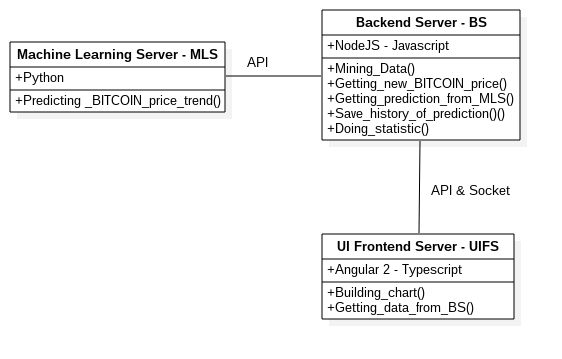
\includegraphics[height=3.5in, keepaspectratio=true]{system.png}
\caption{System Structure}
\end{figure}\\

\subsection{Hệ thống Machine Learning Server}
Đây là hệ thống cốt lõi của của sản phẩm, nó đảm nhiệm khối chức năng dựa vào 
các tham số được truyền vào để đưa ra giá trị nhãn tương ứng cho bộ tham số 
đó.\\\\
Cụ thể, để đưa ra một dự đoán, hệ thống yêu cầu các tham số đầu vào phải được 
xây dựng theo mô tả của Feature Selection - 12 features.\\\\
Trong hệ thống Machine Learning Server, được chia nhỏ thành hai phần:\\
\begin{enumerate}
\item Prediction: bao gồm các chức năng đọc mô hình Multilayer Neural Network 
đã xây dựng, chạy mô hình với tham số truyền vào và lấy các kết quả đầu ra.
Kết quả đầu ra có giá trị nhãn Up-Down và xác suất dự đoán.
\item Django: bao gồm các chức năng để hình thành một API server ví dụ như 
tiếp nhận các yêu cầu thông qua API, phản hồi các yêu cầu...
\end{enumerate}
Vì tính chất hỗ trợ tốt cho Machine Learning nên Python được lựa chọn là ngôn 
ngữ để phát triển hệ thống này.\\\\
\subsection{ Hệ thống Backend Server}
Vì bản thân hệ thống Machine Learning Server không có các khối chức năng 
liên quan đến việc  
lấy dữ liệu giá BITCOIN cũng như khai phá dữ liệu nên hệ thống Backend Server
được xây dựng để thực hiện các chức năng này. Đồng thời, Backend Server còn là 
cầu nối giữa trải nghiệm người dùng (hệ thống UI Frontend Server) và hệ thống 
Machine Learning Server.\\\\
Để thực hiện được công việc trên, hệ thống bao gồm được xây dựng các chức năng:\\
\begin{enumerate}
\item Cập nhật giá BITCOIN: thông qua các public API được các sàn giao dịch 
BITCOIN cung cấp, các hàm lấy giá được chạy liên tục để cập nhật giá BITCOIN 
mới nhất nhằm phục vụ cho quá trình dự đoán.
\item Khai phá dữ liệu: dữ liệu được các hàm cập nhật giá BITCOIN lấy được vẫn 
còn ở dạng thô, chưa qua xử lý. Khai phá dữ liệu là biến đổi các dữ liệu này 
về các bộ tham số có ý nghĩa với Machine Learning, các giá trị này mới đích thực 
dùng để làm đầu vào dự đoán xu hướng giá trị BITCOIN.
\item Giao tiếp với hệ thống Machine Learning Server: truyền tham số đi và nhận 
kết quả trả về từ hệ thống Machine Learning Server thông qua API.
\item Lưu trữ và thống kê dữ liệu: thực hiện việc lưu trữ dữ liệu, từ đó tạo nên 
một hệ thống các dữ liệu phục vụ cho việc phân tích, thống kê để cung cấp cho người 
dùng đầu cuối. Đó là các thông tin hết sức quý giá phục vụ cho các nhà đầu tư.
\item Giao tiếp với hệ thống UI Frontend Server: đưa ra những API chức năng nhằm 
phục vụ cho UI Frontend Server. Ví dụ như: yêu cầu dữ liệu dự đoán, yêu cầu 
thống kê đúng/sai, yêu cầu dữ liệu giá cho biểu đồ...
\end{enumerate}
Với khả năng xử lý nhanh, được hỗ trợ tốt nên NodeJS được dùng để phát triển 
hệ thống. Đồng thời, cơ sở dữ liệu của hệ thống là MongoDB vì tính linh hoạt 
trong cấu trúc dữ liệu và khả năng mở rộng cao.\\\\
\subsection{Hệ thống UI Frontend Server}
Hệ thồng UI Frontend Server là một giao diện người dùng, nó cho phép người 
dùng có thể tiếp cận với các chức năng của toàn bộ hệ thống một cách dễ dàng. 
Hệ thống bao gồm nhiều biểu đồ, cũng như tham số cung cấp các thông tin có ý 
nghĩa đầu tư - dự đoán xu hướng giá trị BITCOIN - đồng thời với đó, là các 
thông tin về độ tin cậy của hệ thống, các thống kê về lịch sử dự đoán...\\\\
Một số hình ảnh về hệ thống thực tế.\\
\begin{figure}[h!]
\centering
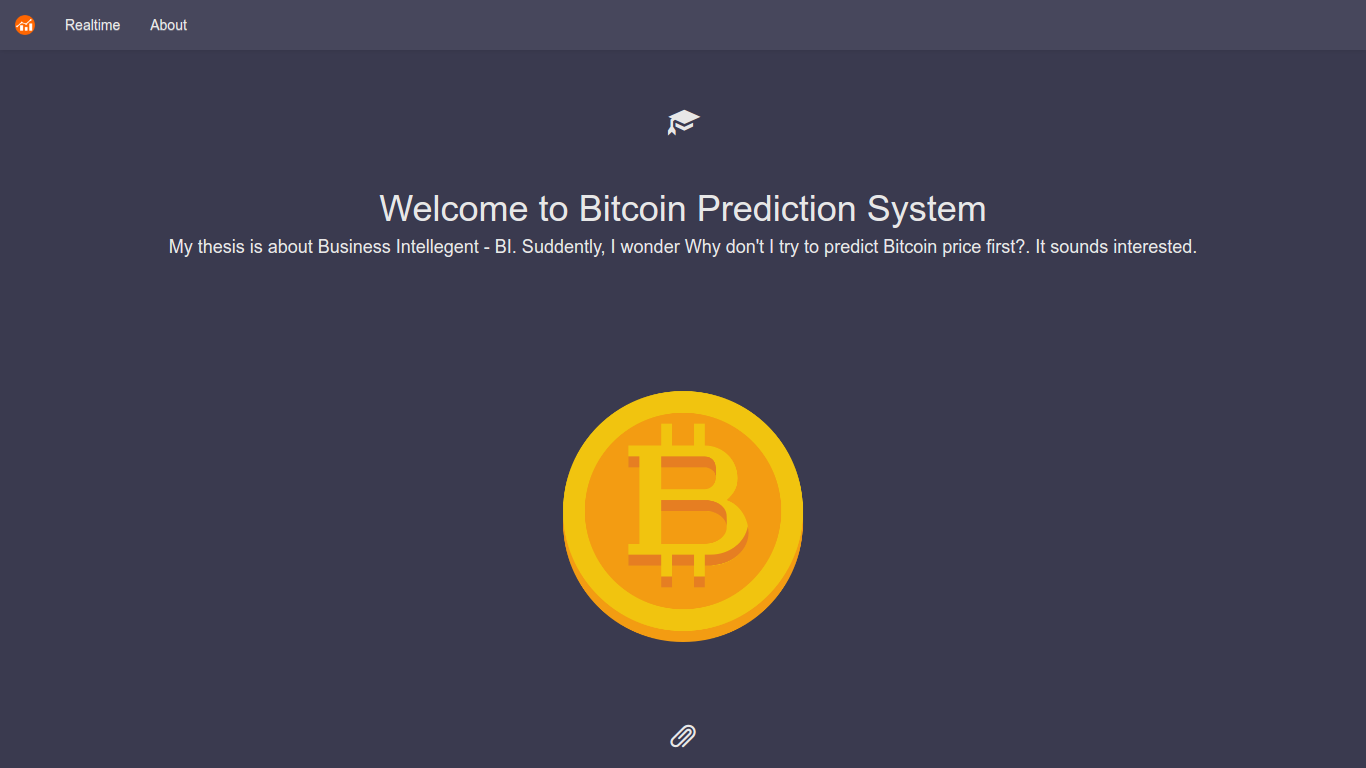
\includegraphics[height=3in, keepaspectratio=true]{1.png}
\caption{UI Frontend Server 1}
\end{figure}\\
\begin{figure}[h!]
\centering
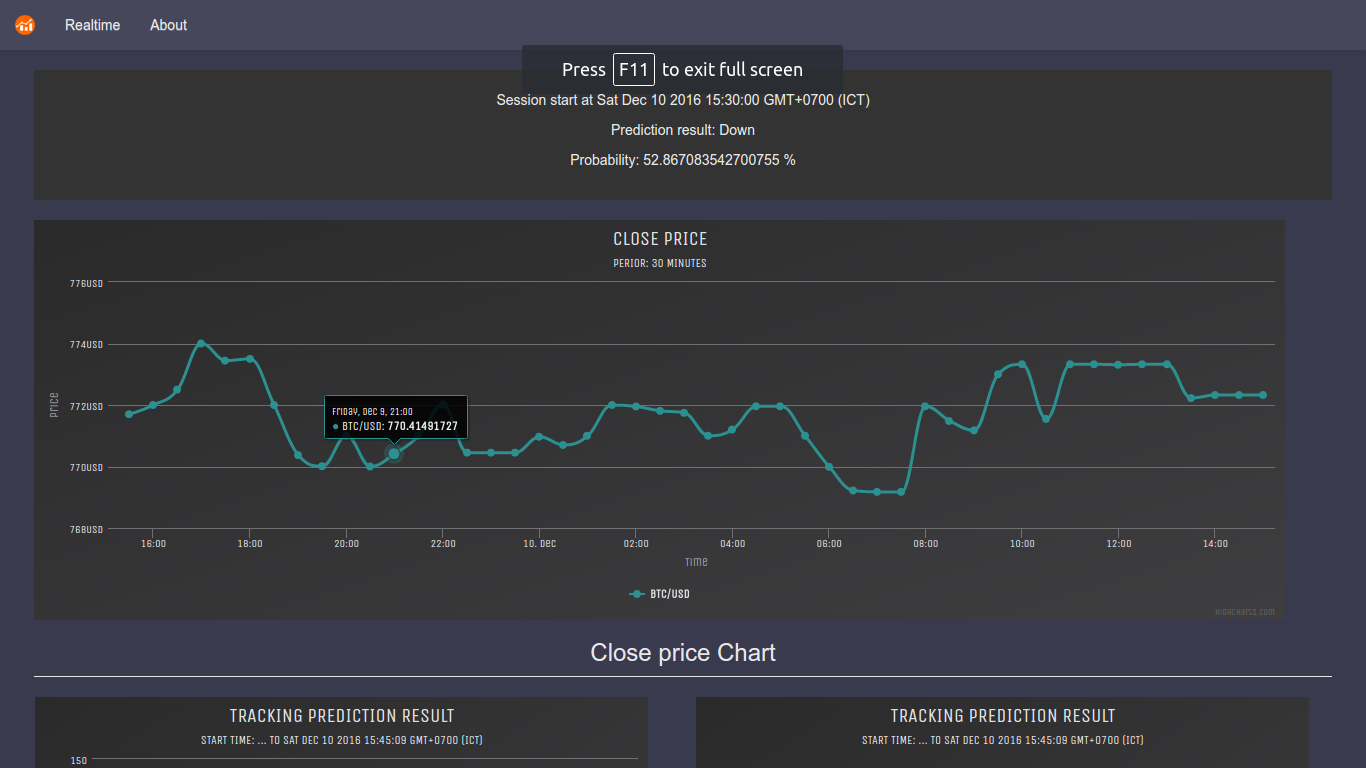
\includegraphics[height=3in, keepaspectratio=true]{2.png}
\caption{UI Frontend Server 2}
\end{figure}\\\\
\begin{figure}[h!]
\centering
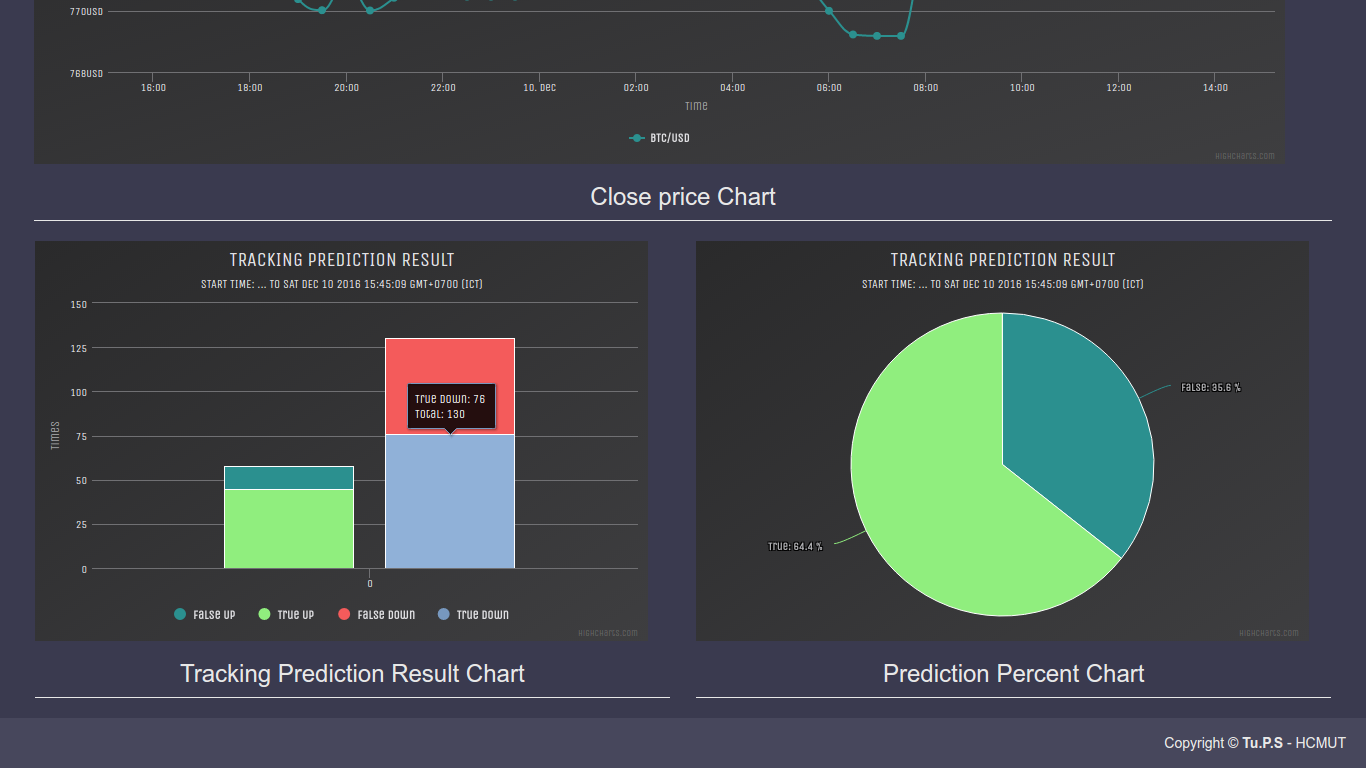
\includegraphics[height=3in, keepaspectratio=true]{3.png}
\caption{UI Frontend Server 3}
\end{figure}\\\\
Hệ thống UI Frontend Server được xây dựng theo xu hướng one-page, cũng chính 
vì vậy mà Angular 2 là lựa chọn phù hợp, với khả năng phát triển nhanh, hỗ trợ 
tốt từ các bên thứ 3.